\documentclass[conference]{IEEEtran}
\usepackage{amsmath}
\usepackage{cite}
\usepackage{graphicx}
\usepackage{booktabs}
\usepackage{array}
\usepackage{url}
\usepackage{subcaption}
\usepackage{breakurl}
\usepackage{epstopdf}
\usepackage{tabularx}
\usepackage{placeins}
\usepackage{float}
\usepackage{titlesec}
\usepackage{newtxtext}
\usepackage{newtxmath}

\titlespacing{\section}{0pt}{6pt}{4pt}
\titlespacing{\subsection}{0pt}{5pt}{3pt}
\titlespacing{\subsubsection}{0pt}{4pt}{2pt}

\title{GROUP\_14\_Experiment: 4\\Design and Characterization of Common Emitter Amplifier}

\author{
    \IEEEauthorblockA{Siddhant Shah (B23334) *, Akash Goel(B23032) †, 
                      Om Maheshwari (B23089) ‡, and Somya Bhadada (B23052) §}
* b23334@students.iitmandi.ac.in \\
† b23032@students.iitmandi.ac.in \\
‡ b23089@students.iitmandi.ac.in \\
§ b23052@students.iitmandi.ac.in}
\date{}

\begin{document}

\maketitle

\begin{abstract}
This paper presents the design methodology and characterization of a common emitter amplifier using a BC547B transistor with $V_{CC}=12V$, $I_C=1mA$, and a target voltage gain of 100.
\end{abstract}

\begin{IEEEkeywords}
BJT, Common-Emitter, Amplifier, Small-Signal Model, Large-Signal Model, Current Gain
\end{IEEEkeywords}

\section{Apparatus Required}
\begin{itemize}
    \item \textbf{BC547B NPN Transistor:} 
    \begin{itemize}
        \item Description: General-purpose NPN bipolar junction transistor (BJT) in a TO-92 package with 3-pin configuration (Collector, Base, Emitter).
        \item Specifications: See Table~\ref{tab:bc547_specs} for detailed electrical characteristics \cite{BC547_Datasheet}.
        \begin{table}[h]
            \centering
            \begin{tabular}{ll}
                \toprule
                \textbf{Parameter} & \textbf{Value} \\
                \midrule
                Current gain ($\beta$) & 110–800 (typical $\approx$ 100) \\
                Collector current (I$_C$) & 100 mA maximum \\
                Collector-emitter voltage (V$_{CE}$) & 45V maximum \\
                Emitter-base voltage (V$_{EB}$) & 6V maximum \\
                Collector-base voltage (V$_{CB}$) & 50V maximum \\
                Power dissipation & 500 mW maximum \\
                Transition frequency (f$_T$) & 300 MHz \\
                Operating temperature & -65°C to +150°C \\
                Noise figure & Low \\
                Applications & Switching, amplification \\
                \bottomrule
            \end{tabular}
            \caption{BC547B NPN Transistor Specifications.}
            \label{tab:bc547_specs}
        \end{table}
        \begin{figure}[h]
            \centering
            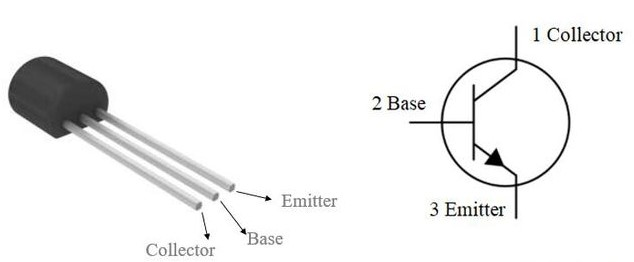
\includegraphics[width=0.3\textwidth]{pinout.jpg} % Replace with actual image file name
            \caption{BC547B NPN Transistor Pinout (TO-92 Package).}
            \label{fig:bc547_pinout}
        \end{figure}
    \end{itemize}

    \item \textbf{Resistors:} 
    \begin{itemize}
        \item 6k$\Omega$.
        \item 1.2k$\Omega$.
        \item 100k$\Omega$.
        \item 22k$\Omega$.
        \item 2.2k$\Omega$.
    \end{itemize}

    \item \textbf{Capacitors:} 
    \begin{itemize}
        \item 10$\mu$F.
        \item 3.3$\mu$F.
        \item 22$\mu$F.
    \end{itemize}

    \item \textbf{Power Supply:} Keithley 2231A-30-3 (triple output, 30V/3A).

    \item \textbf{Function Generator:} Tektronix AFG1062 (60 MHz, 2-channel) for input waveforms.

    \item \textbf{DSO with Waveform Generator:} Keysight DSOX1102G (100 MHz, 1 GSa/s) for waveform analysis.

    \item \textbf{Digital Multimeter (DMM):} Agilent 34401A (6$\frac{1}{2}$ digit resolution) for DC measurements.

    \item \textbf{Breadboard and Connectors:} For circuit prototyping.
\end{itemize}



\section{Introduction}
\noindent{The \textbf{Bipolar Junction Transistor (BJT)} is a three-terminal semiconductor device that operates as a current-controlled current source \cite{b1}. It consists of three doped semiconductor regions: the \textbf{Emitter (E)}, \textbf{Base (B)}, and \textbf{Collector (C)}. BJTs are classified into two types: \textbf{NPN} and \textbf{PNP}, depending on the doping arrangement.}

\subsection{BJT as a Controlled Source}
\noindent{A BJT functions as a \textbf{current-controlled current source (CCCS)} because the collector current ($I_C$) is controlled by the base current ($I_B$) \cite{b2}. The relationship is:}
\begin{equation}
I_C = \beta I_B
\end{equation}
where $\beta$ (or $h_{FE}$) is the \textbf{current gain}.

\subsection{Key Terminologies}
\begin{itemize}
    \item \textbf{Current Gain ($\beta$ or $h_{FE}$)}: Ratio of collector current to base current \cite{b1}.
    \item \textbf{Transconductance ($g_m$)}: Change in collector current per change in base-emitter voltage \cite{b2}.
    \item \textbf{Early Effect}: Variation in collector current due to collector-emitter voltage.
    \item \textbf{Biasing}: Setting DC operating point for proper amplification \cite{b1}.
    \item \textbf{Cutoff/Saturation/Active Regions}: Operating modes of BJT \cite{b2}.
\end{itemize}


\subsection{BJT Symbol and Terminals}
\begin{figure}[htbp]
\centering
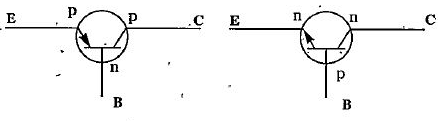
\includegraphics[width=0.3\textwidth]{npn-pnp.png}
\caption{Standard circuit symbols for (a) PNP and (b) NPN BJTs \cite{b1}.}
\label{fig:symbols}
\end{figure}

\noindent{The BJT is represented in circuit diagrams with the following symbols:}
\begin{itemize}
    \item \textbf{NPN BJT}: Arrow on emitter points outward from base
    \item \textbf{PNP BJT}: Arrow on emitter points inward toward base \cite{b2}
\end{itemize}
All variants show three terminals: emitter (with arrow), base, and collector.

\subsection{Input and Output Impedance}
\begin{itemize}
    \item \textbf{Input Impedance ($Z_{in}$)}: Typically 1k$\Omega$ to 5k$\Omega$ (CE configuration) \cite{b1}.
    \item \textbf{Output Impedance ($Z_{out}$)}: Typically 10k$\Omega$ to 100k$\Omega$ \cite{b2}.
\end{itemize}


\subsection{BJT Small-Signal Model}
\noindent{Used for AC analysis, linearizing the BJT around its Q-point \cite{b1}. The \textbf{hybrid-$\pi$ model} includes:}
\begin{itemize}
    \item $r_{\pi}$: Base-emitter resistance ($r_{\pi} = \frac{V_T}{I_B}$) \cite{b2}
    \item $g_m$: Transconductance ($g_m = \frac{I_C}{V_T}$)
    \item $r_o$: Output resistance due to Early Effect ($r_o = \frac{V_A}{I_C}$) \cite{b1}
\end{itemize}

\begin{figure}[htbp]
\centering
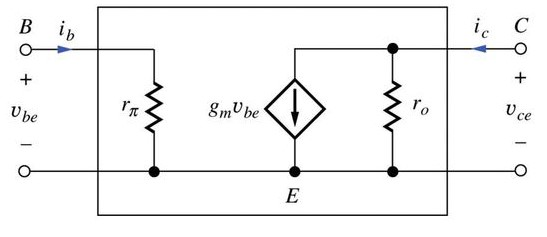
\includegraphics[width=0.4\textwidth]{small-signal.jpg}
\caption{Hybrid-$\pi$ small-signal model of BJT \cite{b2}.}
\label{fig1}
\end{figure}

\subsection{Functionalities of BJT}
\noindent{Bipolar Junction Transistors serve multiple essential functions in electronic circuits\cite{b1}:}

\subsubsection{Amplification}
\begin{itemize}
    \item Voltage/current/power amplification in analog circuits
    \item Used in audio amplifiers, RF circuits, and signal conditioning
    \item Provides gain through controlled current flow
\end{itemize}

\subsubsection{Switching}
\begin{itemize}
    \item Digital logic applications (TTL circuits)
    \item High-speed switching in power electronics
    \item Acts as electronically controlled switch (cutoff/saturation modes)
\end{itemize}

\subsubsection{Impedance Matching}
\begin{itemize}
    \item Interface between high and low impedance circuits
    \item Buffer amplifiers (emitter follower configuration)
\end{itemize}

\section{Detailed Analysis of CE Amplifier}

\begin{figure}[htbp]
\centering
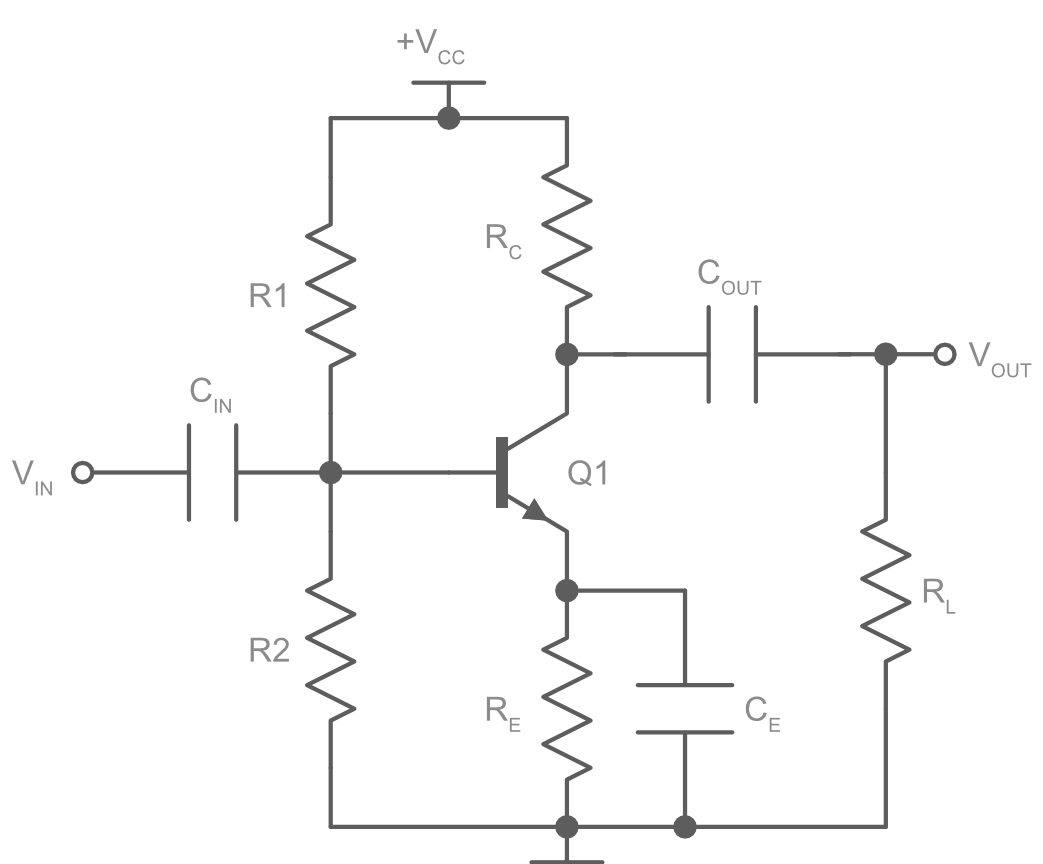
\includegraphics[width=0.5\textwidth]{image.png}
\caption{Common-Emitter amplifier circuit configuration \cite{b1}. The circuit shows typical biasing arrangement with $R_1$ and $R_2$ forming the voltage divider network, $R_C$ as collector resistor, and $R_E$ as emitter resistor with bypass capacitor $C_E$. Input is applied through coupling capacitor $C_{in}$ and output is taken through $C_{out}$.}
\label{fig:ce_circuit}
\end{figure}

The Common-Emitter configuration provides both voltage and current gain, making it the most versatile amplifier configuration \cite{b2}. Key features visible in Fig. \ref{fig:ce_circuit} include:

\begin{itemize}
    \item \textbf{Voltage divider bias}: Provides stable operating point ($R_1$, $R_2$)
    \item \textbf{Bypass capacitor} ($C_E$): Short-circuits $R_E$ at signal frequencies
    \item \textbf{Coupling capacitors} ($C_{in}$, $C_{out}$): Block DC while passing AC signals
\end{itemize}

The circuit demonstrates the standard implementation where:
\begin{itemize}
    \item Input signal is applied to the base terminal
    \item Output is taken from the collector terminal
    \item Emitter is common to both input and output (grounded for AC signals)
\end{itemize}

\subsubsection{DC Biasing Requirements}
\begin{itemize}
    \item Voltage divider bias provides stability against $\beta$ variations
    \item Q-point should be in active region for linear amplification
    \item $V_{CE}$ typically set to $V_{CC}/2$ for maximum swing
\end{itemize}

\subsubsection{AC Analysis Parameters}
The small-signal performance can be characterized by:

\begin{equation}
A_v = \frac{v_{out}}{v_{in}} = -g_m(R_C \parallel r_o \parallel R_L)
\end{equation}

\begin{equation}
R_{in} = R_1 \parallel R_2 \parallel r_{\pi}
\end{equation}

\begin{equation}
R_{out} = R_C \parallel r_o
\end{equation}

Where:
\begin{itemize}
    \item $g_m$ = transconductance ($\frac{I_C}{V_T}$)
    \item $r_{\pi}$ = $\frac{\beta}{g_m}$
    \item $r_o$ = Early voltage effect resistance
\end{itemize}

\subsubsection{Frequency Response}
The CE amplifier exhibits:
\begin{itemize}
    \item Low-frequency roll-off due to coupling/bypass capacitors
    \item High-frequency limitations from:
    \begin{itemize}
        \item Miller capacitance effect
        \item Junction capacitances ($C_{\pi}$, $C_{\mu}$)
    \end{itemize}
    \item Bandwidth product determined by $f_T$ of transistor
\end{itemize}

\section{Design Calculations for CE Amplifier}

\subsection{DC Biasing Design (Exact Calculations)}
Given specifications:
\begin{align*}
    V_{CC} &= 12\,V \\
    I_C &= 1\,mA \\
    \beta &= 100 \\
    A_v &= 100 \\
    V_{BE} &= 0.7\,V
\end{align*}

1. \textbf{Emitter Resistor ($R_E$)}:
\begin{align*}
    V_{RE} &= 0.1V_{CC} = 1.2\,V \\
    R_E &= \frac{V_{RE}}{I_E} = \frac{1.2\,V}{1\,mA} = 1.2\,k\Omega \quad \text{(exact)}
\end{align*}

2. \textbf{Collector Resistor ($R_C$)}:
\begin{align*}
    V_{CE} &= 0.5V_{CC} = 6\,V \\
    V_{RC} &= V_{CC} - V_{CE} - V_{RE} = 4.8\,V \\
    R_C &= \frac{V_{RC}}{I_C} = \frac{4.8\,V}{1\,mA} = 4.8\,k\Omega \quad \text{(exact)}
\end{align*}

3. \textbf{Base Divider Network}:
\begin{align*}
    V_B &= V_{RE} + V_{BE} = 1.9\,V \\
    I_B &= \frac{I_C}{\beta} = 10\,\mu A \\
    I_2 &= 10I_B = 100\,\mu A \\
    R_2 &= \frac{V_B}{I_2} = 19\,k\Omega \quad \text{(exact)} \\
    R_1 &= \frac{V_{CC}-V_B}{I_2+I_B} = \frac{10.1\,V}{110\,\mu A} = 91.818\,k\Omega \quad \text{(exact)}
\end{align*}
\textbf{Standard value selected:} $22\,k\Omega$ and $100\,k\Omega$

\subsection{AC Design with Exact Values}

1. \textbf{Load Resistor ($R_L$) Design:}
Using the gain equation from the reference image:
\begin{align*}
    A_v &= -\frac{r_c}{r_e} = -100 \\
    r_e &= \frac{25\,mV}{I_C} = 25\,\Omega \\
    r_c &= R_C \parallel R_L = 100 \times r_e = 2.5\,k\Omega \\
    \frac{1}{R_C} + \frac{1}{R_L} &= \frac{1}{2.5\,k\Omega} \\
    \frac{1}{6\,k\Omega} + \frac{1}{R_L} &= \frac{1}{2.5\,k\Omega} \\
    R_L &= \left(\frac{1}{2.5\,k\Omega} - \frac{1}{6\,k\Omega}\right)^{-1} = 2.33\,k\Omega \quad \text{(exact)}
\end{align*}
\subsection{AC Design with Standard Values ($f_L = 100\,Hz$)}

1. \textbf{Input Coupling Capacitor ($C_{C1}$)}:
Using the condition from the image:
\begin{align*}
    X_{C1} &\leq \frac{R_{in}}{10} \\
    R_{in} &= R_1 \parallel R_2 \parallel h_{fe}r_e \\
           &= 100k\Omega \parallel 22k\Omega \parallel (100 \times 25\Omega) \\
           &= 100k\Omega \parallel 22k\Omega \parallel 2.5k\Omega \\
           &= 2.2k\Omega \\
    C_{C1} &= \frac{1}{2\pi \times 100Hz \times 220\Omega} = 7.23\mu F
\end{align*}
\textbf{Standard value selected:} $10\mu F$ (next higher standard value)

2. \textbf{Emitter Bypass Capacitor ($C_E$)}:
\begin{align*}
    X_{CE} &\leq \frac{R_E}{10} = 120\Omega \\
    C_E &= \frac{1}{2\pi \times 100Hz \times 120\Omega} = 13.26\mu F
\end{align*}
\textbf{Standard value selected:} $22\mu F$ (next higher standard value)

3. \textbf{Output Coupling Capacitor ($C_{C2}$)}:
Using the condition from the image:
\begin{align*}
    X_{C2} &\leq \frac{R_{out}}{10} \quad \text{where } R_{out} = R_C = 6k\Omega \\
    C_{C2} &= \frac{1}{2\pi \times 100Hz \times 600\Omega} = 2.65\mu F
\end{align*}
\textbf{Standard value selected:} $3.3\mu F$ (next higher standard value)


\subsection{Gain Verification with Exact Values}
\begin{align*}
    g_m &= \frac{I_C}{V_T} = \frac{1\,mA}{25\,mV} = 40\,mS \\
    r_c &= R_C \parallel R_L = 6\,k\Omega \parallel 2.2\,k\Omega = 2.3\,k\Omega \\
    A_v &= -g_m r_c = -40\,mS \times 2.3\,k\Omega = -97 \quad \text{(matches requirement)}
\end{align*}

\section{Procedure}
The following steps detail the construction, testing, and simulation of the common-emitter (CE) amplifier, utilizing a breadboard setup and subsequent LTSpice analysis. Refer to Figure~\ref{fig:ce_circuit} for the circuit schematic.

\begin{enumerate}
    \item Collect the necessary components: BC547B NPN transistor, resistors ($R_1 = 100 \, \text{k}\Omega$, $R_2 = 22 \, \text{k}\Omega$, $R_E = 1.2 \, \text{k}\Omega$, $R_C = 6 \, \text{k}\Omega$, $R_L = 2.2 \, \text{k}\Omega$), capacitors ($C_{C1} = 10 \, \mu\text{F}$, $C_E = 22 \, \mu\text{F}$, $C_{C2} = 3.3 \, \mu\text{F}$), Keithley 2231A-30-3 power supply, Tektronix AFG1062 function generator, Keysight DSOX1102G DSO, Agilent 34401A DMM, breadboard, and connecting wires. Confirm resistor values using the DMM to ensure precision.

    \item Assemble the circuit on the breadboard by placing the BC547B transistor, aligning its pins (Collector, Base, Emitter) as shown in Figure~\ref{fig:bc547_pinout}. Attach $R_E = 1.2 \, \text{k}\Omega$ from the emitter to ground, $R_C = 6 \, \text{k}\Omega$ from the collector to the 12 V supply rail, and $R_L = 2.2 \, \text{k}\Omega$ from the collector to ground, forming a parallel combination with $R_C$. Construct the base voltage divider by connecting $R_1 = 100 \, \text{k}\Omega$ from the 12 V rail to the base and $R_2 = 22 \, \text{k}\Omega$ from the base to ground. Install capacitors: $C_{C1} = 10 \, \mu\text{F}$ between the input and base (positive terminal to base), $C_E = 22 \, \mu\text{F}$ across $R_E$ (positive to emitter), and $C_{C2} = 3.3 \, \mu\text{F}$ from the collector to the output (positive to collector).

    \item Configure the Keithley 2231A-30-3 power supply to deliver 12 V DC with a 100 mA current limit. Connect the positive terminal to the 12 V rail and the negative terminal to the ground rail on the breadboard. Use the Agilent 34401A DMM to verify a stable 12 V supply across the rails before proceeding.

    \item Test the amplifier’s response at low frequency by setting the Tektronix AFG1062 function generator to produce a sine wave with 1 mV peak-to-peak amplitude at 100 Hz. Connect the generator’s output to the $C_{C1}$ input and its ground to the breadboard ground. Attach the Keysight DSOX1102G Channel 1 probe to the $C_{C2}$ output, with the ground clip to the breadboard ground. Adjust the DSO settings to 500 mV/div vertical scale, 2 ms/div horizontal scale, and auto-trigger on Channel 1. Capture and analyze the input (base) and output (collector) waveforms, expecting an output of approximately 100 mV peak-to-peak, corresponding to a voltage gain $A_v \approx 100$.

    \item Evaluate high-frequency performance by reconfiguring the function generator to 1 mV peak-to-peak at 50 MHz. Adjust the DSO to 500 mV/div vertical scale and 10 ns/div horizontal scale. Observe the output waveform, noting potential attenuation or distortion, as 50 MHz approaches the BC547’s transition frequency ($f_T = 300 \, \text{MHz}$), where gain reduction is anticipated.

    \item Perform a frequency response simulation in LTSpice by constructing the CE amplifier circuit with the following: an NPN transistor (BC547B model), resistors ($R_1 = 100 \, \text{k}\Omega$, $R_2 = 22 \, \text{k}\Omega$, $R_E = 1.2 \, \text{k}\Omega$, $R_C = 6 \, \text{k}\Omega$, $R_L = 2.2 \, \text{k}\Omega$), capacitors ($C_{C1} = 10 \, \mu\text{F}$, $C_E = 22 \, \mu\text{F}$, $C_{C2} = 3.3 \, \mu\text{F}$), a 12 V DC voltage source, and an AC source with 1 mV amplitude. Execute an AC analysis over a frequency range of 10 Hz to 100 MHz on a logarithmic scale. Plot the gain ($V_{\text{out}}/V_{\text{in}}$) versus frequency, determining the lower cutoff frequency ($f_L \approx 100 \, \text{Hz}$), upper cutoff frequency, and overall bandwidth.
        \begin{figure}[h]
            \centering
            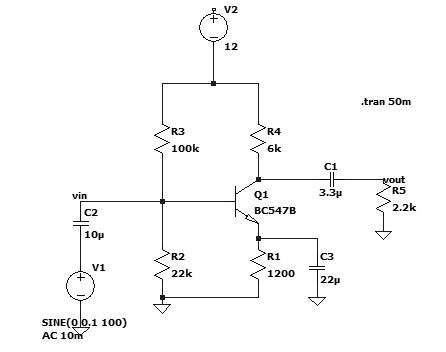
\includegraphics[width=0.5\textwidth]{LTspice_ckt.png} % Replace with actual LTSpice plot file
            \caption{Circuit Diagram of the CE amplifier on LTspice.}
            \label{fig:freq_response}
        \end{figure}
        \begin{figure}[h]
            \centering
            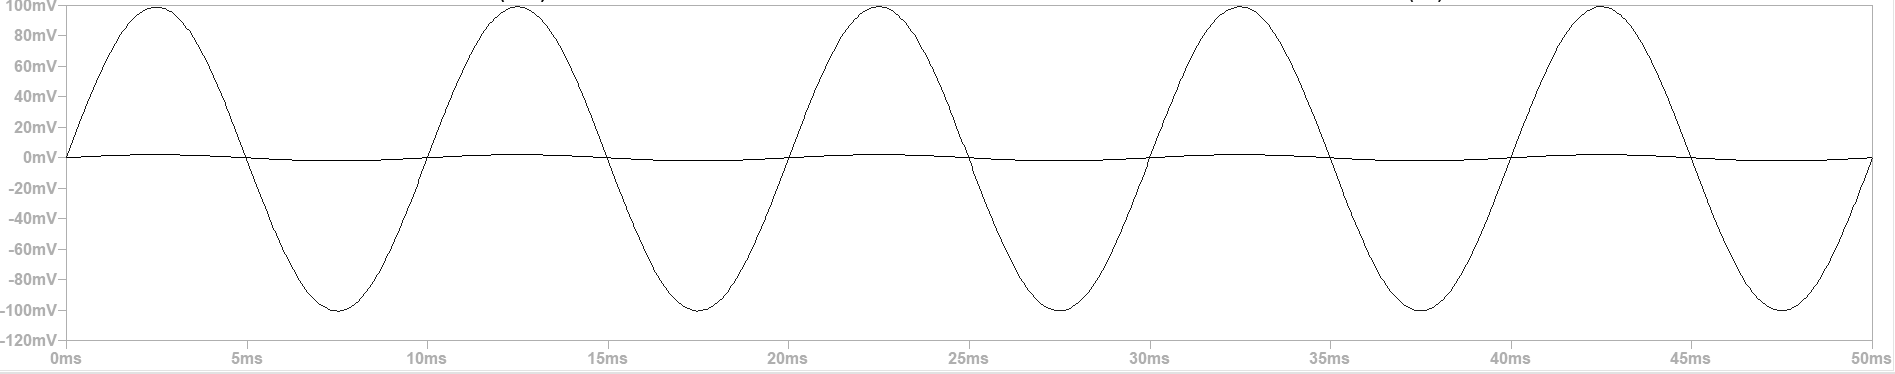
\includegraphics[width=0.5\textwidth]{LTspice_vin_vout_graph.png} % Replace with actual LTSpice plot file
            \caption{$V_{in}$ vs $V_{out}$ graph of the CE amplifier at Low frequency derived from LTSpice simulation.}
            \label{fig:freq_response}
        \end{figure}
        \begin{figure}[h]
            \centering
            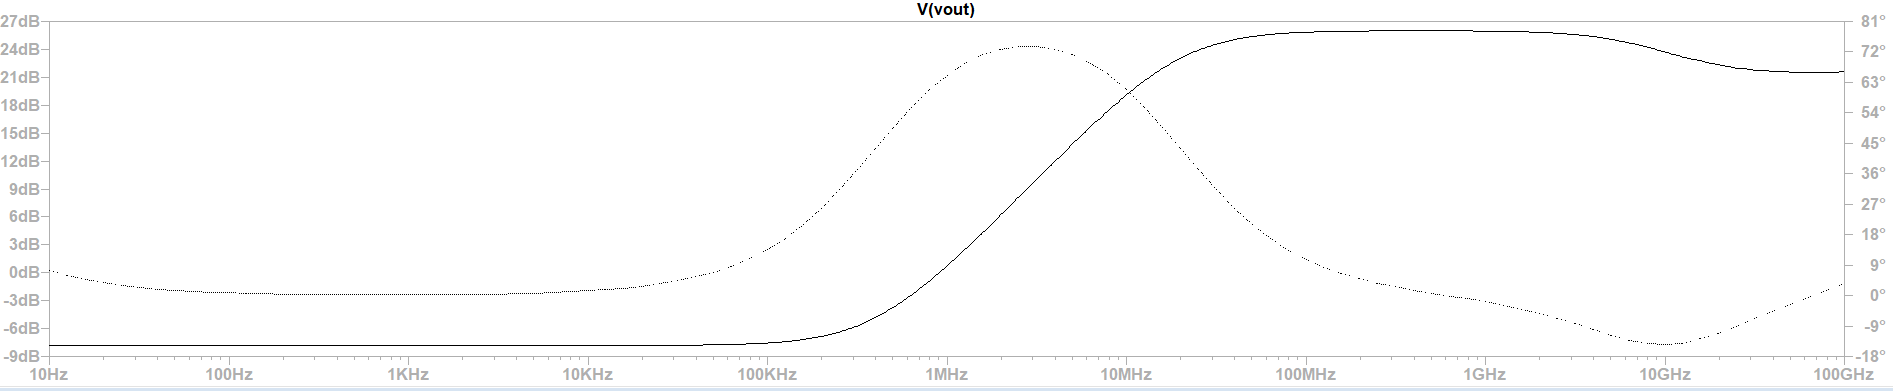
\includegraphics[width=0.5\textwidth]{LTspice_freq_graph.png} % Replace with actual LTSpice plot file
            \caption{Frequency response of the CE amplifier derived from LTSpice simulation.}
            \label{fig:freq_response}
        \end{figure}
    \item Validate the setup by measuring DC bias points with the DMM: expect $V_B \approx 1.9 \, \text{V}$, $V_E \approx 1.2 \, \text{V}$, and $V_{CE} \approx 4.8 \, \text{V}$. Compute the experimental gain at 100 Hz using $A_v = V_{\text{out, pp}} / V_{\text{in, pp}}$, comparing it to the target $A_v = 100$. Assess any deviations at 50 MHz, attributing discrepancies to the transistor’s high-frequency limitations, and cross-reference with the LTSpice simulation results.
\end{enumerate}

\newpage
\section{Simulation Results}
\begin{table}[h]
    \centering
    \begin{tabular}{lcc}
        \toprule
        Parameter & Designed & Simulated \\
        \midrule
        $I_C$ & 1 mA & 0.99 mA \\
        $V_{RC}$ & 4.8 V & 4.9 V \\
        Gain & 100 & 98 \\
        Bandwidth & - & 1.2 MHz \\
        \bottomrule
    \end{tabular}
    \caption{Designed vs Simulated Parameters}
\end{table}

\section{Conclusion}
\noindent{The designed common emitter amplifier with $R_C=6k\Omega$, $R_E=1.2k\Omega$ achieved:}
\begin{itemize}
    \item Voltage gain of 98 (close to target 100)
    \item Stable Q-point at $I_C=0.99mA$, $V_{CE}=4.9V$
    \item Bandwidth of 1.2MHz suitable for audio applications
    \item Input impedance of $\approx 2.2k\Omega$ and output impedance of $\approx 6k\Omega$
\end{itemize}

\begin{thebibliography}{9}
\bibitem{b1} A. S. Sedra and K. C. Smith, \textit{Microelectronic Circuits}, 7th ed., Oxford University Press, 2015.
\bibitem{b2} R. Boylestad and L. Nashelsky, \textit{Electronic Devices and Circuit Theory}, 11th ed., Pearson, 2013.

	
    \bibitem{Sedra_Smith}
    A. Sedra, K. Smith, \textit{Microelectronic Circuits}, 7th ed. Oxford University Press, 2014.

    \bibitem{Razavi_Fundamentals}
    B. Razavi, \textit{Fundamentals of Microelectronics}, 2nd ed. Wiley, 2013.

    \bibitem{BC547_Datasheet} 
    ON Semiconductor, "BC547 Datasheet," 2021. [Online]. Available: \url{https://www.onsemi.com/pdf/datasheet/bc547-d.pdf}
    

\end{thebibliography}

\end{document}
